\documentclass[11pt,a4paper]{article}
\usepackage[margin=2.2cm]{geometry}
\usepackage[T1]{fontenc}
\usepackage{charter}
\usepackage{microtype}
\usepackage{graphicx}
\usepackage{booktabs}
\usepackage{array}
\usepackage{tabularx}
\usepackage{float}
\usepackage{caption}
\usepackage{enumitem}
\usepackage{amsmath}
\usepackage[table]{xcolor}
\usepackage{listings}
\usepackage[most]{tcolorbox}
\usepackage{fancyhdr}
\usepackage[colorlinks=true,linkcolor=accent,urlcolor=accent]{hyperref}

\definecolor{accent}{HTML}{3C3489}
\definecolor{codebg}{HTML}{F6F6F3}
\definecolor{kw}{HTML}{185FA5}
\definecolor{cm}{HTML}{6B6A64}
\definecolor{okgreen}{HTML}{0F6E56}
\definecolor{badred}{HTML}{A32D2D}

\setlength{\parindent}{0pt}
\setlength{\parskip}{6pt}
\setlist{itemsep=2pt,topsep=4pt}
\captionsetup{font=small,labelfont=bf}
\renewcommand{\arraystretch}{1.18}

\pagestyle{fancy}\fancyhf{}
\rhead{\small\color{cm}\reporttag}
\cfoot{\small\thepage}
\renewcommand{\headrulewidth}{0.3pt}

\lstdefinelanguage{SV}{
  morekeywords={module,endmodule,input,output,inout,logic,wire,reg,always_ff,always_comb,assign,
    begin,end,if,else,case,endcase,default,typedef,enum,localparam,posedge,negedge,or,task,endtask,
    function,endfunction,automatic,initial,repeat,while,for,integer,string,signed,void},
  sensitive=true, morecomment=[l]{//}, morecomment=[s]{/*}{*/}, morestring=[b]"}
\lstdefinelanguage{DCTcl}{
  morekeywords={set,lappend,define_design_lib,analyze,elaborate,current_design,link,check_design,
    create_clock,set_input_delay,set_output_delay,set_max_area,compile,report_area,report_timing,
    report_qor,report_resources,report_constraints,write,write_sdc,set_dont_use,get_lib_cells,puts,gui_start},
  sensitive=true, morecomment=[l]{\#}}
\lstset{basicstyle=\ttfamily\footnotesize, backgroundcolor=\color{codebg}, frame=single,
  rulecolor=\color{codebg}, keywordstyle=\color{kw}\bfseries, commentstyle=\color{cm}\itshape,
  columns=fullflexible, keepspaces=true, breaklines=true, showstringspaces=false,
  xleftmargin=4pt, xrightmargin=4pt, aboveskip=6pt, belowskip=6pt}

\newtcolorbox{task}{colback=accent!5,colframe=accent,boxrule=0.6pt,arc=2pt,
  left=8pt,right=8pt,top=4pt,bottom=4pt,fonttitle=\bfseries,title=The assignment}
\newtcolorbox{keypoint}[1]{colback=okgreen!6,colframe=okgreen,boxrule=0.6pt,arc=2pt,
  left=8pt,right=8pt,top=4pt,bottom=4pt,fonttitle=\bfseries,title={#1}}
\newtcolorbox{lesson}[1]{colback=orange!7,colframe=orange!70!black,boxrule=0.6pt,arc=2pt,
  left=8pt,right=8pt,top=4pt,bottom=4pt,fonttitle=\bfseries,title={#1}}

\newcommand{\fig}[3]{\begin{figure}[H]\centering\includegraphics[width=#2\linewidth]{figures/#1}\caption{#3}\end{figure}}
\newcommand{\pass}{\textcolor{okgreen}{\textbf{PASS}}}
\newcommand{\met}{\textcolor{okgreen}{\textbf{MET}}}
\newcommand{\viol}{\textcolor{badred}{\textbf{VIOLATED}}}

\newcommand{\header}[3]{%
  \begin{center}
  {\small\color{cm} CPE 527 VLSI Design \quad|\quad Lab 2 \quad|\quad University of Alabama in Huntsville}\\[8pt]
  {\LARGE\bfseries\color{accent} #1}\\[4pt]
  {\large #2}\\[8pt]
  {\small Bibek Shrestha \quad|\quad September 2026 \quad|\quad #3}
  \end{center}\vspace{2pt}\hrule\vspace{6pt}}
\newcommand{\reporttag}{Lab 2 / Assignment 1: Fibonacci generator synthesis}
\begin{document}
\header{Synthesizing a 16-bit Fibonacci Generator}{Speed vs.\ area experiments and the critical path}{Synopsys VCS + Design Compiler, SAED 90\,nm}

\begin{task}
Use the SystemVerilog Fibonacci generator from Lab 1. Synthesize it with the flow from the tutorial.
Experiment with different optimizations (for speed or for area). Verify that the synthesized design
passes the Lab 1 testbench. Generate area and speed reports. \textbf{What is the critical path in your design?}
\end{task}

\section*{At a glance}
\begin{table}[H]\centering\small
\begin{tabular}{lccc}
\toprule
 & \textbf{Baseline} & \textbf{Speed} & \textbf{Area} \\
\midrule
Clock target & 5 ns & 3 ns & 5 ns \\
Effort (map / area) & medium / medium & high / low & medium / high \\
Critical path delay & 4.35 ns & 3.01 ns & 4.35 ns \\
Slack & +0.56 ns \met & $-0.09$ ns \viol & +0.56 ns \met \\
Total area & 2759.82 & 3302.43 & 2750.85 \\
Cells & 122 & 201 & 122 \\
Adder built as & ripple carry & NAND2/NAND3 chain & ripple carry \\
\bottomrule
\end{tabular}
\caption{Results of the three synthesis runs.}
\end{table}

\begin{keypoint}{Answer: the critical path}
\texttt{current\_reg[1]} $\rightarrow$ 16-bit ripple-carry adder \texttt{r53} (14 full adders + XOR for bit 15)
$\rightarrow$ enable mux \texttt{AO22X1} $\rightarrow$ \texttt{OUT\_reg[15]}.
Delay 4.35\,ns, slack +0.56\,ns at 5\,ns, so the design can run at about \textbf{225\,MHz}.
\end{keypoint}

\section{The design}
FIBO outputs 1, 1, 2, 3, 5, 8, 13, \dots\ on a 16-bit bus. It has a clock, an asynchronous reset
\texttt{rst}, and an enable \texttt{en}. Each enabled clock does:
\begin{lstlisting}[language=SV]
previous <= current;
current  <= current + previous;
OUT      <= current + previous;
\end{lstlisting}

\fig{a1_block.png}{0.82}{What the RTL turns into: three 16-bit registers (48 flip-flops) and one shared adder.}

\begin{table}[H]\centering\small
\begin{tabular}{ccccc}
\toprule
Cycle & previous & current & sum & OUT \\
\midrule
1 & 1 & 0 & 1 & 1 \\
2 & 0 & 1 & 1 & 1 \\
3 & 1 & 1 & 2 & 2 \\
4 & 1 & 2 & 3 & 3 \\
5 & 2 & 3 & 5 & 5 \\
6 & 3 & 5 & 8 & 8 \\
7 & 5 & 8 & 13 & 13 \\
\bottomrule
\end{tabular}
\caption{How the registers step through the sequence after reset.}
\end{table}

\section{Workflow}
\fig{flow.png}{0.85}{The flow used in all Lab 2 assignments.}

\begin{enumerate}
\item \textbf{Functional simulation} of the RTL with the Lab 1 testbench.
\item \textbf{Synthesis} with one script, \texttt{fibo\_flow.tcl}. Four lines at the top pick the variant,
      and every report and netlist gets the variant name, so runs never overwrite each other.
\item \textbf{Reports}: area, timing, QoR, resources and constraints for each run.
\item \textbf{Gate-level simulation} of the netlist with the same testbench.
\item \textbf{Design Vision} to look at the synthesized circuit.
\end{enumerate}

\begin{lstlisting}[language=bash]
vcs -sverilog -full64 src/assignment2.sv src/assignment2_tb.sv -o f_sim/fibo.simv
./f_sim/fibo.simv
dc_shell -f fibo_flow.tcl            # once per variant
\end{lstlisting}

\textbf{Constraints used:} clock period $T$ (5 or 3\,ns), input and output delay $0.4T$,
\texttt{set\_max\_area 0}, library \texttt{saed90nm\_typ}.

\section{RTL simulation}
\begin{table}[H]\centering\small
\begin{tabular}{cccl}
\toprule
Time (ns) & en & OUT & Note \\
\midrule
0, 1 & 0 & 0 & reset, then idle \\
3, 7, 9, 11 & 1 & 1, 2, 3, 5 & counting \\
13 & 0 & 5 & held (en = 0) \\
15, 17 & 1 & 8, 13 & counting again \\
19 & 0 & 0 & final reset \\
\bottomrule
\end{tabular}
\caption{The RTL gives the right sequence, including the hold.}
\end{table}

\section{Synthesis results}
\subsection*{Area}
\begin{table}[H]\centering\small
\begin{tabular}{lrrr}
\toprule
 & Baseline & Speed & Area \\
\midrule
Combinational area & 1070.90 & 1570.41 & 1065.37 \\
Flip-flop (non-comb.) area & 1547.37 & 1547.37 & 1547.37 \\
Net area & 141.55 & 184.66 & 138.11 \\
\textbf{Total area} & \textbf{2759.82} & \textbf{3302.43} & \textbf{2750.85} \\
Comb.\ / sequential cells & 72 / 48 & 151 / 48 & 72 / 48 \\
\bottomrule
\end{tabular}
\caption{Area reports. The 48 flip-flops cost the same in every run; only the logic changes.}
\end{table}

\subsection*{Timing}
Slack is simply the time left over before the clock edge:
\[
\text{slack} = (T - t_\text{setup}) - t_\text{arrival}
\qquad\Rightarrow\qquad
(5 - 0.09) - 4.35 = +0.56\ \text{ns}
\]
\fig{a1_budget.png}{0.9}{Where the time goes on the critical path in each run.}

The report lists the path gate by gate. Each full adder adds about 0.27\,ns, and there are 14 of them in a row:
\begin{lstlisting}
current_reg[1]/Q (DFFARX1)      0.19    0.19
r53/U1_1/CO (FADDX1)            0.39    0.58
r53/U1_2/CO (FADDX1)            0.27    0.85
   ... 11 more full adders, 0.27 each ...
r53/U1_14/CO (FADDX1)           0.26    4.07
r53/U1_15/Q (XOR3X1)            0.14    4.21
U27/Q (AO22X1)                  0.11    4.32
OUT_reg[15]/D (DFFARX1)         0.03    4.35
slack (MET)                             0.56
\end{lstlisting}

\fig{a1_path.png}{0.8}{Arrival time along the critical path: ripple adder (blue) vs.\ the faster chain DC built for 3\,ns (orange).}

\subsection*{Other things the reports showed}
\begin{itemize}
\item \textbf{One adder, not two.} The resources report maps both \texttt{current + previous} expressions
      onto one \texttt{DW01\_add} (\texttt{rpl} = ripple).
\item \textbf{Mixed reset cells.} \texttt{previous} resets to 1, so bit 0 uses a set-type flip-flop
      (\texttt{DFFASX1}) and bits 1 to 15 use clear-type ones (\texttt{DFFARX1}).
\item \textbf{\texttt{max\_area} VIOLATED is normal.} Asking for zero area can never be met; it just means ``as small as possible''.
\item \texttt{check\_design}: one harmless LINT-1 warning (an unused cell removed by compile).
\end{itemize}

\section{Speed vs.\ area}
\fig{a1_tradeoff.png}{0.88}{Area and delay of each run. Dashed lines are the required times.}

\begin{itemize}
\item \textbf{Speed run:} to aim for 3\,ns, DC replaced the ripple adder with a faster NAND-based carry chain.
      The path got \textbf{31\% faster} (4.35 $\rightarrow$ 3.01\,ns) but the design got \textbf{20\% bigger}
      and used 79 more cells. It still missed 3\,ns by 0.09\,ns.
\item \textbf{Area run:} timing was already met, so there was little to remove: only 9 units saved.
\end{itemize}

\section{Gate-level simulation}
\begin{lstlisting}[language=bash]
vcs -sverilog -full64 -debug_access+all src/assignment2_tb.sv output/fibo_area_synth.v \
    .../verilog/saed90nm.v -o ps_sim/fibo_synth.vsim
./ps_sim/fibo_synth.vsim
\end{lstlisting}

\begin{table}[H]\centering\small
\begin{tabular}{cccc}
\toprule
Time (ns) & RTL OUT & Gate-level OUT & \\
\midrule
3 & 1 & 0 & one cycle late \\
7 / 9 / 11 & 2 / 3 / 5 & 1 / 2 / 3 & one cycle late \\
17 & 13 & 8 & one cycle late \\
19 & 0 & 0 & 13 never appears \\
\bottomrule
\end{tabular}
\caption{The netlist gives the right values, but one clock later than the RTL.}
\end{table}

\textbf{Why:} the testbench changes \texttt{en} and \texttt{rst} right after \texttt{@(posedge clk)},
on the \emph{same} edge where the flip-flops read them. It is a tie, and the RTL and gate-level flip-flop
models break the tie differently. From that edge on the netlist runs one cycle behind, and the final reset
arrives before 13 is captured. This is a testbench issue, not a synthesis bug.

\fig{a1_race.png}{0.85}{The same input edge is read differently by the two models.}

\begin{lesson}{Fix}
Change inputs on the falling edge (\texttt{@(negedge clk)}), as the Assignment 2 and 3 testbenches do.
Their gate-level runs match the RTL exactly. Also, a 5\,ns clock in the testbench would match the synthesis target.
\end{lesson}

\section{Design Vision}
\begin{figure}[H]\centering
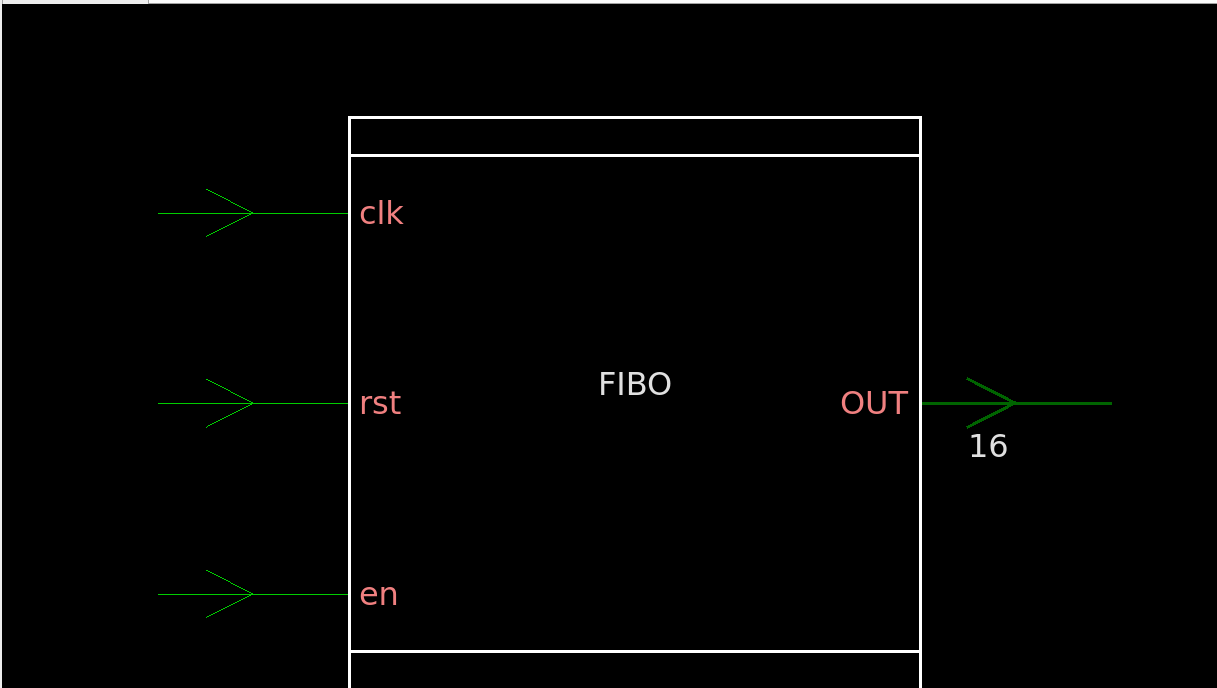
\includegraphics[width=0.42\linewidth]{figures/a1_dv_symbol.png}\hfill
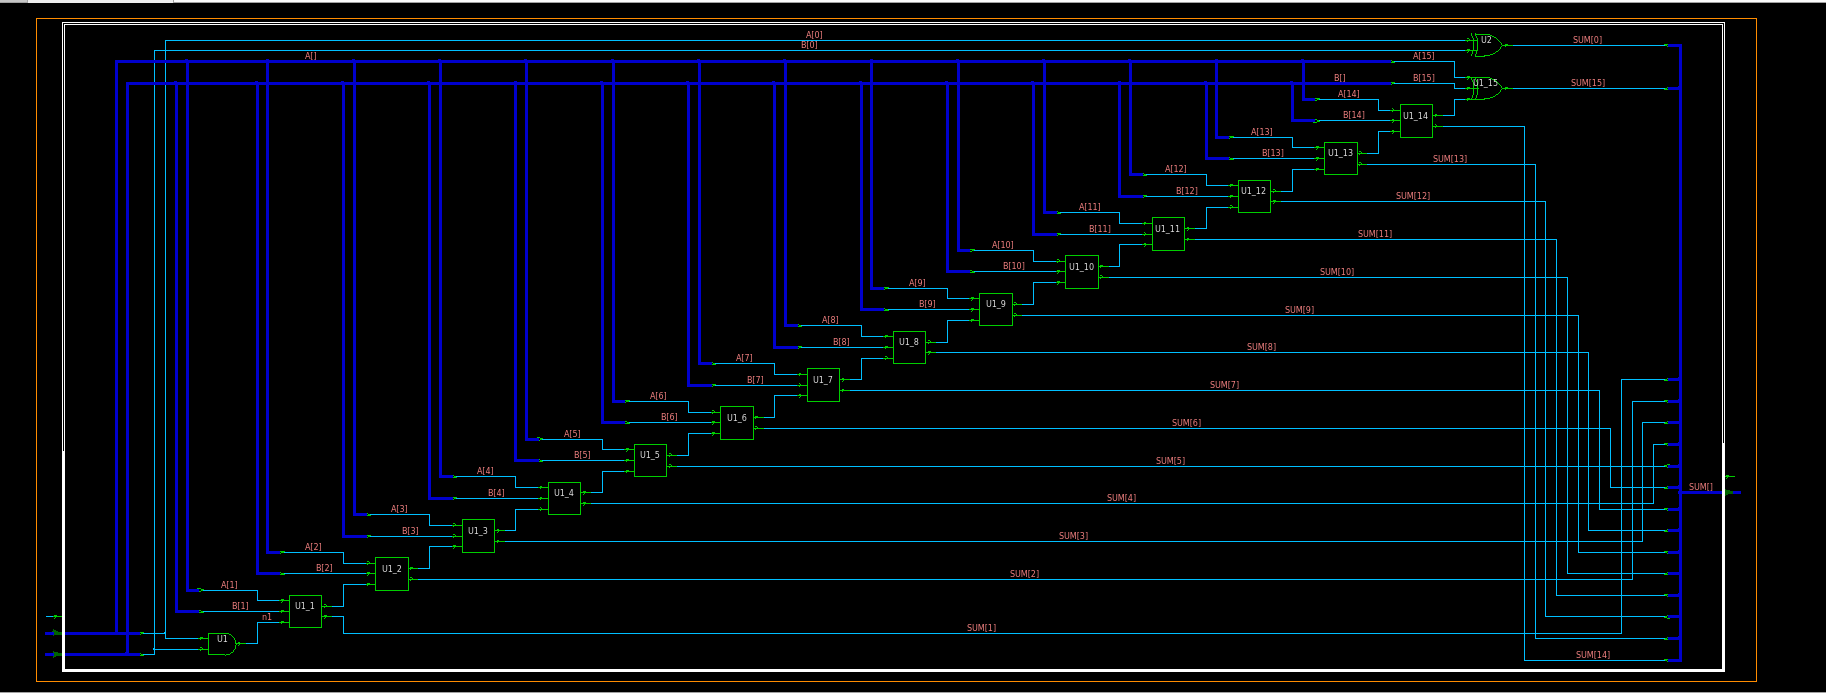
\includegraphics[width=0.55\linewidth]{figures/a1_dv_adder_gates.png}
\caption{Left: synthesized FIBO block. Right: gates of the shared adder; the diagonal staircase is the carry chain (the critical path).}
\end{figure}

\section{What I learned}
\begin{itemize}
\item The clock target decides the hardware: the same code gave a ripple adder at 5\,ns and a faster adder at 3\,ns.
\item Speed costs area: 31\% faster cost 20\% more area.
\item Flip-flops are a fixed cost; synthesis can only optimize the logic.
\item A clean timing report does not guarantee a clean simulation. The testbench must not change inputs on the sampling edge.
\end{itemize}

\appendix
\section{Source files}
\subsection*{RTL: \texttt{src/assignment2.sv}}
\lstinputlisting[language=SV]{src/assignment2.sv}
\subsection*{Testbench: \texttt{src/assignment2\_tb.sv}}
\lstinputlisting[language=SV]{src/assignment2_tb.sv}
\subsection*{Synthesis script: \texttt{src/fibo\_flow.tcl}}
\lstinputlisting[language=DCTcl]{src/fibo_flow.tcl}
\end{document}
